\documentclass[10pt]{article}
\usepackage{fullpage}
\usepackage{enumitem}
\usepackage{amsmath}
\usepackage{amssymb}
\usepackage{graphicx}
\usepackage[T1]{fontenc}
\usepackage{lipsum}
\usepackage{listings}
\usepackage{float}
\usepackage{scrextend}
\usepackage{hyperref}
\usepackage{algorithmicx}
\usepackage{algpseudocode}
\usepackage{tikz}
\usepackage{pgfplots}
\usetikzlibrary{arrows,
                backgrounds,
                fit,
                positioning,
                quotes,
                shapes,
                pgfplots.colorbrewer,
}
                
\usepackage{xcolor}
\usepackage{wrapfig}
\usepackage[demo]{graphicx}
\usepackage{subcaption}
\usepackage[section]{placeins}
\usepackage{float}% If comment this, figure moves to Page 2


\pgfplotsset{
    cycle from colormap manual style/.style={
        x=3cm,y=10pt,ytick=\empty,
        stack plots=y,
        every axis plot/.style={line width=2pt},
    },
}

%\pagecolor[rgb]{0,0,0}
%\pagecolor[rgb]{0.0549,0.0667,0.0862}

\iffalse
\pagecolor[rgb]{0.1269, 0.1369, 0.1469}
\color[rgb]{1,1,1}

\fi

\newenvironment{subs}
  {\adjustwidth{3em}{0pt}}
  {\endadjustwidth}

\title{\vspace{-1cm} \Huge Project 1 \\ \LARGE CmpE 300, Analysis of Algorithms, Fall 2022 }
\author{
    Bahadır Gezer - 2020400039 \\
    Muhammet Batuhan Ilhan - 2019400243 \\
}
\date{November 2022}

\begin{document}
\maketitle
  
\tableofcontents
\clearpage


\section{Theoretical Analysis}

\begin{quote}
\begin{algorithmic}[1]
\Require $n = 2^{k}-1$, $k \in \mathbb{Z}^{+}$
\Require $arr[i] \in \{0,1,2\}$, $0 \leq i \leq n-1$
\State $\textbf{Input: } arr[0:n-1]$ 
\State $\textbf{Output: } arr2[0:4]$ 
\State $\textbf{function }Example(arr[0:n-1])$
\State 
\State $arr2 \gets [0,0,0,0,0]$
\For {$i \gets 0 \textbf{ to } n-1$}
    \If{$arr[i] = 0$}
        \For {$t1 \gets i \textbf{ to } n-1$}
            \State $p1 \gets t1^{1/2}$
            \State $x1 \gets n + 1$
            \While{$x1 \geq 1$}
                \State $x1 \gets \lfloor x1 / 2 \rfloor$
                \State $arr2[i \bmod 5] \gets arr2[i \bmod 5] + 1$
            \EndWhile
        \EndFor
    \ElsIf{$arr[i] = 1$}
        \For{$t2 \gets n \textbf{ down to } 1$}
            \For{$p2 \gets 1 \textbf{ to } n$}
                \State $x2 \gets n + 1$
                \While{$x2 > 0$}
                    \State $x2 \gets \lfloor x2 / 2 \rfloor$
                    \State $arr2[i \bmod 5] \gets arr2[i \bmod 5] + 1$
                \EndWhile
            \EndFor
        \EndFor
    \ElsIf{$arr[i] = 2$}
        \For{$t3 \gets 1 \textbf{ to } n$}
            \State $x3 \gets t3 + 1$
            \For{$p3 \gets 0 \textbf{ to } t3^{2} - 1$}
                \State $arr2[i \bmod 5] \gets arr2[i \bmod 5] + 1$
            \EndFor
        \EndFor
    \EndIf
\EndFor
\State $\textbf{end}$
\end{algorithmic}
\end{quote}

\begin{description}
   \item[for loop 1 - line 6:] This loop will iterate \textbf{from} $0$ \textbf{to}  $\mathbf{n-1}$. Which is a total of $\mathbf{n}$ iterations. 
   
   \item[for loop 2 - line 8:] This loop will iterate \textbf{from} $\mathbf{i}$ \textbf{to}  $\mathbf{n-1}$. Which is a total of $\mathbf{n-i}$ iterations. 

    \begin{align*}
    i &= 0 \text{\hspace{0.5cm}loop iterates n times} \\
    i &= 1 \text{\hspace{0.5cm}loop iterates n - 1 times}\\
    i &= 2 \text{\hspace{0.5cm}loop iterates n - 2 times}\\
    &\vdots \\
    i &= n - 1 \text{\hspace{0.5cm}loop iterates 1 time} \\
    \end{align*}

    Therefore, this loop iterates $\mathbf{\frac{n \cdot (n+1)}{2}}$ times. This calculation takes for loop 1 into account.

   \item[while loop 1 - line 11:] This loop will iterate \textbf{from} $\mathbf{n+1}$ \textbf{to} $\mathbf{1}$ by halving at each iteration. For the sake of simplicity, lets consider $\mathbf{n+1}$ as $\mathbf{2^{z}}$ where $\mathbf{z}$ is some positive integer. It will be generalized using interpolation later.
   \begin{enumerate}[leftmargin=3cm]
       \item[\textit{\textbf{Iteration 1 -}}] ${k = 2^{z}}$
       \item[\textit{\textbf{Iteration 2 -}}] ${k = 2^{z-1}}$
       \item[\textit{\textbf{Iteration 3 -}}] ${k = 2^{z-2}}$
       \item[]\hspace{-1.5cm}\textbf{\vdots}\hspace{2cm}\textbf{\vdots}
       \item[\textit{\textbf{Iteration m -}}] ${k = 2^{z-m-1} = 1}$
   \end{enumerate}
  As seen above, the loop will iterate $\mathbf{m}$ times. Solving the equation $\mathbf{2^{z-m-1} = 1}$ for $\mathbf{m}$ we get $\mathbf{m = z - 1}$. Substituting $\mathbf{z = log_2(n+1)}$ into the equation we get $\mathbf{m = log_2(n+1) - 1}$. Thus, the loop will have $\mathbf{log_2(n+1) - 1}$ iterations. The last iteration does not count, because of the termination statement of the while loop, so the real number of iterations is $\mathbf{log_2(n+1) - 2}$.

    \item[for loop 3 - line 17:] This loop will iterate \textbf{from} $\mathbf{n}$ \textbf{to}  $\mathbf{1}$. The loop is not interrupted mid iteration. Thus the total number of iterations come out to be $\mathbf{n}$. 

    \item[for loop 4 - line 18:] This loop will iterate \textbf{from} $\mathbf{1}$ \textbf{to}  $\mathbf{n}$. The loop is not interrupted mid iteration. Thus the total number of iterations come out to be $\mathbf{n}$. 

   \item[while loop 2 - line 20:] This loop will iterate \textbf{from} $\mathbf{n+1}$ \textbf{to} $\mathbf{1}$ by halving at each iteration. For the sake of simplicity, lets consider $\mathbf{n+1}$ as $\mathbf{2^{z}}$ where $\mathbf{z}$ is some positive integer. 
   \begin{enumerate}[leftmargin=3cm]
       \item[\textit{\textbf{Iteration 1 -}}] ${k = 2^{z}}$
       \item[\textit{\textbf{Iteration 2 -}}] ${k = 2^{z-1}}$
       \item[\textit{\textbf{Iteration 3 -}}] ${k = 2^{z-2}}$
       \item[]\hspace{-1.5cm}\textbf{\vdots}\hspace{2cm}\textbf{\vdots}
       \item[\textit{\textbf{Iteration m -}}] ${k = 2^{z-m-1} = 1}$
   \end{enumerate}
 As seen above, the loop will iterate $\mathbf{m}$ times. Solving the equation $\mathbf{2^{z-m-1} = 1}$ for $\mathbf{m}$ we get $\mathbf{m = z - 1}$. Substituting $\mathbf{z = log_2(n+1)}$ into the equation we get $\mathbf{m = log_2(n+1) - 1}$. Thus, the loop will have $\mathbf{log_2(n+1) - 1}$ iterations. \par


\item[for loop 5 - line 27:] This loop will iterate \textbf{from} $\mathbf{1}$ \textbf{to} $\mathbf{n}$. The loop is not interrupted mid iteration. Thus the total number of iterations come out to be $\mathbf{n}$. 

\item[for loop 6 - line 29:] This loop will iterate \textbf{from} $\mathbf{0}$ \textbf{to} $\mathbf{t3^2-1}$. 
    \begin{align*}
    t3 &= 0 \text{\hspace{0.5cm}loop iterates $\mathbf{0^{2}}$ times} \\
    t3 &= 1 \text{\hspace{0.5cm}loop iterates $\mathbf{1^{2}}$ times}\\
    t3 &= 2 \text{\hspace{0.5cm}loop iterates  $\mathbf{2^{2}}$ times}\\
    &\vdots \\
    t3 &= n - 1 \text{\hspace{0.5cm}loop iterates $\mathbf{(n-1)^{2}}$ time} \\
    \end{align*}
Since there is no interruption in the loop, it will always iterate ($\mathbf{0^2 +1^2 + 2^2 + ... + (n -1)^2}$) times. This sum is equal to $\mathbf{\frac{(n-1) \cdot n \cdot (2n-1) } {6} }$. This value is the total number of times the statements inside this loop will iterate, it takes the outer loop into account. \par
\end{description}

\iffalse
We have three if blocks, and the program executes one of them in each iteration of the most outer for loop. Each if block has constant iteration number because loops have no interruption and loop conditions does not depend on input except size of the input.\par
\begin{description}
\item[first if block  - line 7:] This block includes two loops, for loop 2 and while loop 1. While loop 1 is in the for loop 2. For loop 2 iterates $\mathbf{\frac{n \cdot (n -1)} {2} }$ times, and for each iteration of the for loop, while loop 2 iterates $\mathbf{m = log_2(n+1) - 1}$ times. Therefore, total execution number of the statements inside the while loop 1 is  $\mathbf{(\frac{n \cdot (n -1)} {2}) \cdot (log_2(n+1) - 1)}$ 

\item[second if block  - line 16:] This block includes three loops, for loop 3, for loop 4 and while loop 2. While loop 2 is in the for loop 4, and for loop 4 is in the for loop 3. For loop 3 iterates $\mathbf{n}$ times, and for each iteration of the for loop 3, for loop 4 iterates $\mathbf{n}$ times. For each iteration of the for loop 4, while loop 2 iterates $\mathbf{m = log_2(n+1) - 1}$ times. Therefore, total execution number of the statements inside the while loop 2 is  $\mathbf{ n^2 \cdot (log_2(n+1) - 1)}$ 

\item[third if block  - line 26:] This block includes two loops, for loop 5 and for loop 6. For loop 6 is in the for loop 5. For loop 5 iterates $\mathbf{n}$ times, and for each iteration of the for loop 5, for loop 6 iterates  $\mathbf{\frac{(n-1) \cdot n \cdot (2n-1) } {6} }$ times. Therefore, total execution number of the statements inside the for loop 6 is $\mathbf{\frac{ n^2\cdot (n-1) \cdot (2n-1) } {6} }$
\end{description}
\fi


\subsection{Comparison as Basic Operation - (1)}

\indent \indent Since for loop 1 runs without interruption - we do not have any break statements. So the the comparison will run regardless of the input. This comparison will be executed once for each iteration of the for loop. This loop will iterate \textbf{from} $\mathbf{0}$ \textbf{to} $\mathbf{n-1}$, which is $\mathbf{n}$ iterations. 

\subsubsection{Analyze \textit{B(n)}}
\indent \indent The complexity does not matter on the input. The loop iterates $\mathbf{n}$ times, and the comparison is executed once for each iteration of the loop. Thus, $\mathbf{B(n) = 1 \cdot n}$. We can prove that this complexity belongs to the  $\mathbf{\Theta(n)}$ complexity class by using the definitions of $\boldsymbol{\mathcal{O}}$ and $\mathbf{\Omega}$

\begin{align*}
B(n) &= n \le n &\\
 &\implies B(n) \in \mathcal{O}(n) &\\
B(n) &= n \ge n &\\
 &\implies B(n) \in \Omega(n) &\\
 B(n) \in \Omega(n) \land B(n) \in \mathcal{O}(n) &\implies \mathbf{B(n) \boldsymbol{\in} \Theta(n)} &\\
 & &\Box
\end{align*}

\subsubsection{Analyze \textit{W(n)}}
\indent \indent The complexity does not matter on the input. The loop iterates $\mathbf{n}$ times, and the comparison is executed once for each iteration of the loop. Thus, $\mathbf{W(n) = 1 \cdot n}$. We can prove that this complexity belongs to the  $\mathbf{\Theta(n)}$ complexity class by using the definitions of $\boldsymbol{\mathcal{O}}$ and $\mathbf{\Omega}$

\begin{align*}
W(n) &= n \le n &\\
 &\implies W(n) \in \mathcal{O}(n) &\\
W(n) &= n \ge n &\\
 &\implies W(n) \in \Omega(n) &\\
 W(n) \in \Omega(n) \land W(n) \in \mathcal{O}(n) &\implies \mathbf{W(n) \boldsymbol{\in} \Theta(n)} &\\
 & &\Box
\end{align*}


\subsubsection{Analyze \textit{A(n)}}
\indent \indent The complexity does not matter on the input. The loop iterates $\mathbf{n}$ times, and the comparison is executed once for each iteration of the loop. Thus, $\mathbf{A(n) = 1 \cdot n}$. We can prove that this complexity belongs to the  $\mathbf{\Theta(n)}$ complexity class by using the definitions of $\boldsymbol{\mathcal{O}}$ and $\mathbf{\Omega}$

\begin{align*}
A(n) &= n \le n &\\
 &\implies A(n) \in \mathcal{O}(n) &\\
A(n) &= n \ge n &\\
 &\implies A(n) \in \Omega(n) &\\
 A(n) \in \Omega(n) \land A(n) \in \mathcal{O}(n) &\implies \mathbf{A(n) \boldsymbol{\in} \Theta(n)} &\\
 & &\Box
\end{align*}


\subsection{Three Assignments as Basic Operation - (2)}
\label{sec:real}

\indent \indent There are three possible entries in the input set, one for each if statement. The first if statement has one basic operation inside of it. This basic operation runs for loops 1 and 2, and also while loop 1. These are all executing inside of each other, so we will multiply their iteration counts. The basic operation is running once for all of these iterations. The second if statement -branch- also has one basic operation inside of it. This second basic operation runs for loops 1, 3 and 4, and also while loop 2. These are all executing inside of each other, so we will multiply their iteration counts. This second basic operation line runs once for all of these iterations. The third if statement -branch- also has one basic operation inside of it. This third basic operation runs for loop 1, 5 and 6. These are all executing inside of each other, so we will multiply their iteration counts. This third basic operation line runs once for all of these iterations. These executions come out to three entries in the input set, with each of them having a probability of $\frac{1}{3}$. Doing the operations above, we get the input set below. 

\begin{enumerate}[leftmargin=2.6cm]
    \item[\textit{\textbf{$I_{1}$ - }}] $\rho (\mathit{I_{1}}) = \frac{1}{3}$ ,  $\tau (\mathit{I_{1}})= \frac{1}{2} \cdot (n^2 + 1) (log_{2}(1 + n) - 2)$
    \item[\textit{\textbf{$I_{2}$ - }}] $\rho (\mathit{I_{2}}) = \frac{1}{3}$ ,  $\tau (\mathit{I_{2}}) = n^3 \cdot (log_2(n+1) - 1)$
    \item[\textit{\textbf{$I_{3}$ - }}] $\rho (\mathit{I_{3}}) = \frac{1}{3}$ ,  $\tau (\mathit{I_{3}}) = \frac{ n^2\cdot (n-1) \cdot (2n-1) } {6}$
    \item[] $T_{n} = \{I_{1}, I_{2}, I_{3}\}$
\end{enumerate}

\subsubsection{Analyze \textit{B(n)}}
\begin{align*}
B(n) &= min\{\tau(I)\text{ | }I \in T_{n}\} \\
&= \frac{1}{2} \cdot (n^2 - 1) \cdot (log_{2}(n + 1) - 2) \\
&\textit{Some positive constants $\mathbf{c_{1}}$, $\mathbf{c_{2}}$ and $\mathbf{n_{0}}$ can be found such that} \\ 
&\textit{$\mathbf{W(n)}$ is squeezed by the function above when $\mathbf{n > n_{0}}$.} \\
&\implies W(n) \in \Theta (\frac{1}{2} \cdot (n^2 - 1) \cdot (log_{2}(n + 1) - 2)) \\
&\textit{Constants and terms of lower order can be omitted from the complexity class.} \\
&\implies \mathbf{A(n) \boldsymbol{\in} \Theta(n^{2} \cdot log_{2}(n))}
\end{align*}

\subsubsection{Analyze \textit{W(n)}}
\label{sec:thirdif}
\begin{align*}
W(n) &= max\{\tau(I)\text{ | }I \in T_{n}\} \\
&= \frac{ n^2\cdot (n-1) \cdot (2n-1) } {6} \\
&= \frac{n^2}{6} - \frac{n^3}{2} + \frac{n^4}{3} \\
&\textit{Some positive constants $\mathbf{c_{1}}$, $\mathbf{c_{2}}$ and $\mathbf{n_{0}}$ can be found such that} \\ 
&\textit{$\mathbf{W(n)}$ is squeezed by the function above when $\mathbf{n > n_{0}}$.} \\
&\implies W(n) \in \Theta (\frac{n^2}{6} - \frac{n^3}{2} + \frac{n^4}{3}) \\
&\textit{Constants and terms of lower order can be omitted from the complexity class.} \\
&\implies \mathbf{A(n) \boldsymbol{\in} \Theta(n^{4})}
\end{align*}

\subsubsection{Analyze \textit{A(n)}}
\begin{align*}
A(n) &= \displaystyle\sum _{I \in T_{n}} \tau (I) \cdot \rho (I) \\
A(n) &= \frac{1}{3} \cdot \frac{1}{2} \cdot (n^2 - 1) (\log_{2}(1 + n) - 2) + \frac{1}{3} \cdot n^3 (\log_2(n+1) - 1) + \frac{1}{3} \cdot \frac{1} {6} \cdot n^2\cdot (n-1) \cdot (2n-1) \\
&= \frac{n^4}{9} - \frac{n^3}{2} + \frac{n^{3} \log_{2}(n + 1))}{3} - \frac{5 \cdot n^2}{18} + \frac{n^2 \log_{2}(n + 1)}{6} - \frac{\log_{2}(n + 1)}{6} + \frac{1}{3} \\
&\textit{Some positive constants $\mathbf{c_{1}}$, $\mathbf{c_{2}}$ and $\mathbf{n_{0}}$ can be found such that} \\ 
&\textit{$\mathbf{A(n)}$ is squeezed by the function above when $\mathbf{n > n_{0}}$.} \\
&\implies A(n) \in \Theta (\frac{n^4}{9} - \frac{n^3}{2} + \frac{n^{3} \log_{2}(n + 1))}{3} - \frac{5 \cdot n^2}{18} + \frac{n^2 \log_{2}(n + 1)}{6} - \frac{\log_{2}(n + 1)}{6} + \frac{1}{3}) \\
&\textit{Constants and terms of lower order can be omitted from the complexity class.} \\
&\implies \mathbf{A(n) \boldsymbol{\in} \Theta(n^{4})}
\end{align*}


\subsection{Two Assignments as Basic Operation - (3)}
Only second and third if block contains basic operation. The basic operation inside the second if block iterates in while loop 2. Therefore, it has same iteration number with while loop 2 which is $\mathbf{ n^3 \cdot (log_2(n+1) - 1)}$. The basic operation inside the third if block iterates in for loop 6. Therefore, it has same iteration number with for loop 6 which is  $\mathbf{\frac{ n^2\cdot (n-1) \cdot (2n-1) } {6}}$.   

\subsubsection{Analyze \textit{B(n)}}
Best case is where the input array is filled with zeros. In that case the program does not enter the if statements -branches- with our basic operations. Thus, no basic operation is executed when in the best case. So, $\mathbf{B(n) = 0 \cdot n = 0}$, the complexity class of which can be found trivially. $\mathbf{B(n) = \Theta(1)}$.

\subsubsection{Analyze \textit{W(n)}}
Worst case is where the input array is filled with twos. In that case the program only enters the third if branch. In this branch our basic operation is inside of for loops 1, 5 and 6. This same complexity was calculated in \hyperref[sec:thirdif]{\textit{Section 1.2.2}}. So, taking the same steps as before we get $\mathbf{W(n) =\frac{n^2}{6} - \frac{n^3}{2} + \frac{n^4}{3}}$. 
\begin{align*}
W(n) &= \frac{n^2}{6} - \frac{n^3}{2} + \frac{n^4}{3} \\
&\textit{Some positive constants $\mathbf{c_{1}}$, $\mathbf{c_{2}}$ and $\mathbf{n_{0}}$ can be found such that} \\ 
&\textit{$\mathbf{W(n)}$ is squeezed by the function above when $\mathbf{n > n_{0}}$.} \\
&\implies W(n) \in \Theta (\frac{n^2}{6} - \frac{n^3}{2} + \frac{n^4}{3}) \\
&\textit{Constants and terms of lower order can be omitted from the complexity class.} \\
&\implies \mathbf{W(n) \boldsymbol{\in} \Theta(n^{4})}
\end{align*}


\subsubsection{Analyze \textit{A(n)}}
Probabilities of $\mathbf{arr[i]=0 ,arr[i]=1 \text{ and } arr[i]=2}$ are $\boldsymbol{\frac{1}{3}}$. Therefore, each if blocks have same execution probability.
This makes the set $\mathbf{T_{n}}$ have 3 elements. Which each mapping out to one of the three conditional branches the function might enter. 
\begin{enumerate}[leftmargin=2.6cm]
    \item[\textit{\textbf{$I_{1}$ - }}] $\rho (\mathit{I_{1}}) = \frac{1}{3}$ ,  $\tau (\mathit{I_{1}})= 0$
    \item[\textit{\textbf{$I_{2}$ - }}] $\rho (\mathit{I_{2}}) = \frac{1}{3}$ ,  $\tau (\mathit{I_{2}}) = n^3 \cdot (log_2(n+1) - 1)$
    \item[\textit{\textbf{$I_{3}$ - }}] $\rho (\mathit{I_{3}}) = \frac{1}{3}$ ,  $\tau (\mathit{I_{3}}) = \frac{ n^2\cdot (n-1) \cdot (2n-1) } {6}$
\end{enumerate}

\begin{align*}
A(n) &= \displaystyle\sum _{I \in T_{n}} \tau (I) \cdot \rho (I) &&\\
 &= (\frac{1}{3} \cdot 0 + \frac{1}{3} \cdot (n^3 \cdot (log_2(n+1) - 1)) + \frac {1}{3} \cdot \frac{ n^2\cdot (n-1) \cdot (2n-1) } {6} && \\
 &= \frac{n^4}{9} - \frac{n^3}{2} + \frac{n^2}{18} + \frac{n^3log_2(n+1)}{3} && \\ 
 &\textit{Some positive constants $\mathbf{c_{1}}$, $\mathbf{c_{2}}$ and $\mathbf{n_{0}}$ can be found such that} && \\ 
 &\textit{$\mathbf{A(n)}$ is squeezed by the function above when $\mathbf{n > n_{0}}$.} && \\
 &\implies A(n) \in \Theta (\frac{n^4}{9} - \frac{n^3}{2} + \frac{n^2}{18} + \frac{n^3log_2(n+1)}{3}) && \\
 &\textit{Terms of lower order -$\mathbf{n^3, n^2, n^3log_2(n)}$- can be omitted from the complexity class.} && \\
 &\implies \mathbf{A(n) \boldsymbol{\in} \Theta (n^4)} && \\
\end{align*}

\subsection{Two Loop Increments as Basic Operation - (4)}
Only second and third if block contains basic operation. The first basic operation line iterates inside of for loops 1, 3, and 4. These iterations are multiplied together since the loops are all inside of each other. This comes out to a total of $\mathbf{n^{3}}$ iterations. Our first basic operation is executed once for each iteration. So the first basic operation -and the second if block- has a complexity of $\mathbf{n^{3}}$. Our second basic operation line iterates inside of loops 1, and 5. These iterations are multiplied together since the two loops are inside of each other. This comes out to a total of $\mathbf{n^{2}}$ iterations. Our  second basic operation is executed once for each iteration. So the second basic operation - and the third if block- has a complexity of $\mathbf{n^{3}}$. The first if block does not contain any basic operations so it has a basic operation count of $\mathbf{0}$.

\subsubsection{Analyze \textit{B(n)}}
Best case is where the input array is filled with zeros. In that case the program does not enter the if statements -branches- with our basic operations. Thus, no basic operation is executed when in the best case. So, $\mathbf{B(n) = 0 \cdot n = 0}$, the complexity class of which can be found trivially. $\mathbf{B(n) = \Theta(1)}$.

\subsubsection{Analyze \textit{W(n)}}
Worst case is where the input array is filled with ones. In that case the program only enters the second if branch. In this branch our basic operation is inside of for loops 1, 3 and 4. The basic operation count was calculated as $\mathbf{W(n) = n^3}$ above.

\begin{align*}
W(n) &= n^3 \le n^3 &\\
 &\implies W(n) \in \mathcal{O}(n^3) &\\
W(n) &= n^3 \ge n^3 &\\
 &\implies W(n^3) \in \Omega(n^3) &\\
 W(n) \in \Omega(n^3) \land W(n) \in \mathcal{O}(n^3) &\implies \mathbf{W(n) \boldsymbol{\in} \Theta(n^3)} &\\
\end{align*}

\subsubsection{Analyze \textit{A(n)}}
Probabilities of $\mathbf{i}$ in the input array $\mathbf{arr[i]=0 ,arr[i]=1 \text { and } arr[i]=2}$ are $\boldsymbol{\frac{1}{3}}$. Therefore, each if blocks have same execution probability. This makes the set $\mathbf{T_{n}}$ have 3 elements. Which each mapping out to one of the three conditional branches the function might enter. 
\begin{enumerate}[leftmargin=2.6cm]
    \item[\textit{\textbf{$I_{1}$ - }}] $\rho (\mathit{I_{1}}) = \frac{1}{3}$ ,  $\tau (\mathit{I_{1}})= 0$
    \item[\textit{\textbf{$I_{2}$ - }}] $\rho (\mathit{I_{2}}) = \frac{1}{3}$ ,  $\tau (\mathit{I_{2}}) = n^3$
    \item[\textit{\textbf{$I_{3}$ - }}] $\rho (\mathit{I_{3}}) = \frac{1}{3}$ ,  $\tau (\mathit{I_{3}}) = n^2$
\end{enumerate}

\begin{align*}
A(n) &= \displaystyle\sum _{I \in T_{n}} \tau (I) \cdot \rho (I) &&\\
 &= \frac{1}{3} \cdot 0 + \frac{1}{3} \cdot n^3 + \frac{1}{3} \cdot n^2 && \\
 &= \frac{n^3+n^2}{3}&& \\ 
 &\textit{Some positive constants $\mathbf{c_{1}}$, $\mathbf{c_{2}}$ and $\mathbf{n_{0}}$ can be found such that} && \\ 
 &\textit{$\mathbf{A(n)}$ is squeezed by the function above when $\mathbf{n > n_{0}}$.} && \\
 &\implies A(n) \in \Theta (\frac{n^3}{3}+ \frac{n^2}{3}) && \\
&\textit{Constants and terms of lower order can be omitted from the complexity class.} \\
&\implies \mathbf{A(n) \boldsymbol{\in} \Theta (n^3)} && \\
\end{align*}

\subsection{Assignment as Basic Operation - (5)}
Only the first if block contains a basic operation. So the basic operation count for the second and third if block is zero. The basic operation statement in the first if block is iterated inside of for loops 1, and 2. The second for loop iterates without interruption inside of the first one, so the total number of iterations inside of for loop 2 is $\mathbf{\frac{n \cdot (n+1)}{2}}$. The basic operation is executed once for each iteration so the total number of basic operations for the first if block is $\mathbf{\frac{n \cdot (n+1)}{2}}$. 

\subsubsection{Analyze \textit{B(n)}}
Best case is where the input array is either filled with ones or twos. In this case the program does not enter the if statement -branches- with our basic operation, which is the first if block. Thus, no basic operation is executed in the best case. So, $\mathbf{B(n) = 0 \cdot n = 0}$, the complexity class of which can be found trivially. $\mathbf{B(n) = \Theta(1)}$.

\subsubsection{Analyze \textit{W(n)}}
Worst case is where the input array is filled with zeros. In that case the program only enters the first if branch. In this branch our basic operation is inside of for loops 1, and 2. The basic operation count was calculated as $\mathbf{\frac{n \cdot (n+1)}{2}}$ above.

\begin{align*}
W(n) &= \frac{n \cdot (n+1)}{2} &&\\
 &= \frac{n^2}{2} + \frac{n}{2} && \\
 &\textit{Some positive constants $\mathbf{c_{1}}$, $\mathbf{c_{2}}$ and $\mathbf{n_{0}}$ can be found such that} && \\ 
 &\textit{$\mathbf{W(n)}$ is squeezed by the function above when $\mathbf{n > n_{0}}$.} && \\
 &\implies W(n) \in \Theta (\frac{n^2}{2} + \frac{n}{2}) && \\
&\textit{Constants and terms of lower order can be omitted from the complexity class.} \\
&\implies \mathbf{W(n) \boldsymbol{\in} \Theta (n^2)} && \\
\end{align*}

\subsubsection{Analyze \textit{A(n)}}
Probabilities of $\mathbf{arr[i]=0 ,arr[i]=1 \text { and } arr[i]=2}$ are $\boldsymbol{\frac{1}{3}}$. Therefore, each if blocks have same execution probability. This makes the set $\mathbf{T_{n}}$ have 3 elements. Which each mapping out to one of the three conditional branches the function might enter. 

\begin{enumerate}[leftmargin=2.6cm]
    \item[\textit{\textbf{$I_{1}$ - }}] $\rho (\mathit{I_{1}}) = \frac{1}{3}$ ,  $\tau (\mathit{I_{1}})= \frac{n(n-1)}{2}$
    \item[\textit{\textbf{$I_{2}$ - }}] $\rho (\mathit{I_{2}}) = \frac{1}{3}$ ,  $\tau (\mathit{I_{2}}) = 0$
    \item[\textit{\textbf{$I_{3}$ - }}] $\rho (\mathit{I_{3}}) = \frac{1}{3}$ ,  $\tau (\mathit{I_{3}}) = 0$
\end{enumerate}

\begin{align*}
A(n) &= \displaystyle\sum _{I \in T_{n}} \tau (I) \cdot \rho (I) &&\\
 &= \frac{1}{3} \cdot \frac{n(n-1)}{2} + \frac{1}{3} \cdot 0 + \frac{1}{3} \cdot  0 && \\
 &= \frac{n^2}{6} + \frac{n}{6} && \\ 
 &\textit{Some positive constants $\mathbf{c_{1}}$, $\mathbf{c_{2}}$ and $\mathbf{n_{0}}$ can be found such that} && \\ 
 &\textit{$\mathbf{A(n)}$ is squeezed by the function above when $\mathbf{n > n_{0}}$.} && \\
 &\implies A(n) \in \Theta (\frac{n^2}{6} + \frac{n}{6}) && \\
 &\textit{Constants and terms of lower order can be omitted from the complexity class.} \\
 &\implies \mathbf{A(n) \boldsymbol{\in} \Theta (n^2)} && \\
\end{align*}

\section{Identification of Basic Operation(s)}
\label{sec:ident}
The basic operation for this function are the assignment operations to $arr2$. Analysis of this basic operation is already done in \hyperref[sec:real]{\textit{Section 1.2}}.

\newpage
\section{Real Execution}
The real basic operations for this program is identified in \hyperref[sec:ident]{\textit{Section 2}}. Looking at the theoretical analysis -and the results from the real analysis support this- we can say that the best case is where the input array is filled with zeros, the worst case is where the array is filled with twos. The average case has theoretical complexity that is the same as the worst case, but in real analysis we will see lower execution times compared to the worst case. 

\subsection{Best Case}
\begin{center}
\begin{tabular}{|c|c|} 
 \hline
 N Size & Time Elapsed (ms) \\ 
 \hline
 1 & 0.004768372 \\
 \hline
 5 & 0.010967255 \\
 \hline
 10 & 0.031948090 \\
 \hline
 25 & 0.216007233 \\
 \hline
 50 & 1.003980637 \\
 \hline
 75 & 2.583026886 \\
 \hline
 100 & 4.234075546 \\
 \hline
 150 & 10.351896286 \\
 \hline
 200 & 17.199993134 \\
 \hline
 250 & 26.273965836 \\
 \hline
\end{tabular}
\end{center}


\subsection{Worst Case}
\begin{center}
\begin{tabular}{|c|c|} 
 \hline
 N Size & Time Elapsed (ms) \\ 
 \hline
 1 & 0.002861023 \\
 \hline
 5 & 0.026941299 \\
 \hline
 10 & 0.254154205 \\
 \hline
 25 & 8.384943008 \\
 \hline
 50 & 133.820772171 \\
 \hline
 75 & 671.449661255 \\
 \hline
 100 & 2112.159013748 \\
 \hline
 150 & 10967.132091522 \\
 \hline
 200 & 33765.886068344 \\
 \hline
 250 & 83805.630207062 \\
 \hline
\end{tabular}
\end{center}


\subsection{Average Case}
\begin{center}
\begin{tabular}{|c|c|} 
 \hline
 N Size & Time Elapsed (ms) \\ 
 \hline
 1 & 0.006437302 \\
 \hline
 5 & 0.029881795 \\
 \hline
 10 & 0.379641851 \\
 \hline
 25 & 7.709662120 \\
 \hline
 50 & 66.747744878 \\
 \hline
 75 & 334.980964661 \\
 \hline
 100 & 1006.102959315 \\
 \hline
 150 & 4331.564426422 \\
 \hline
 200 & 13257.391373316 \\
 \hline
 250 & 31049.947659175 \\
 \hline
\end{tabular}
\end{center}

\newpage
\section{Comparison}
\subsection{Best Case}
\begin{figure}[H]
\centering
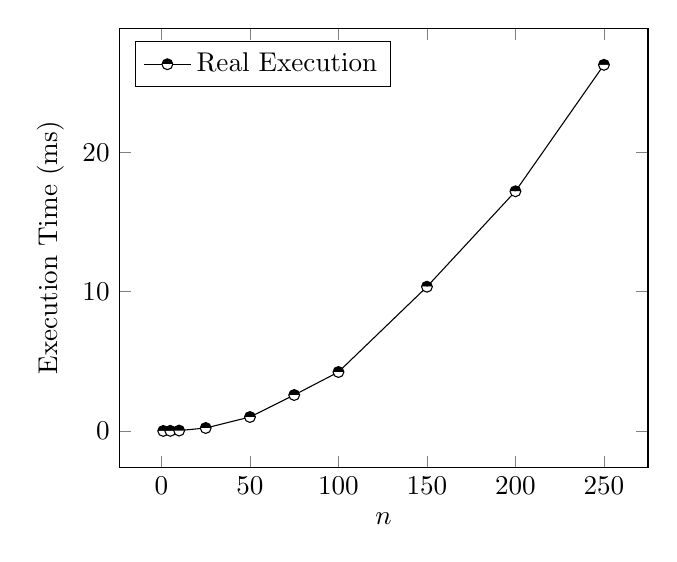
\begin{tikzpicture}[scale = 0.98]
\begin{axis}[grid=minor,
    xlabel=$n$,ylabel=Execution Time (ms), 
    legend pos=north west]
\addplot[
    color=black,
    mark=halfcircle*,
    samples=10,
    ]
    coordinates {(1, 0.004768372)
 (5,0.010967255)
 (10,0.031948090)
 (25,0.216007233)
 (50,1.003980637)
 (75,2.583026886)
 (100,4.234075546)
 (150,10.351896286)
 (200,17.199993134)
 (250,26.273965836)
 };
\addlegendentry{Real Execution}
\end{axis}
\end{tikzpicture}
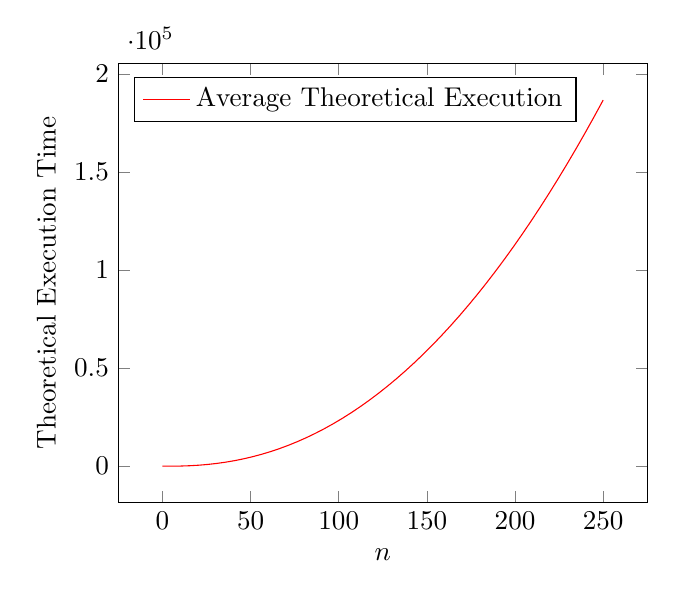
\begin{tikzpicture}[scale = 0.98]
\begin{axis}[grid=minor, xlabel=$n$,ylabel=Theoretical Execution Time,
    legend pos=north west,
    ]
\addplot [color=red, samples = 50, domain=0:250]{(1/2) * (x^2 - 1) * ((ln(x+1)/ln(2)) - 2)};
\addlegendentry{Average Theoretical Execution}
\end{axis}
\end{tikzpicture}
\caption{Side-by-side comparison of the real execution times and the correct theoretical complexity for the best case.}
\end{figure}


\begin{figure}[H]
\centering
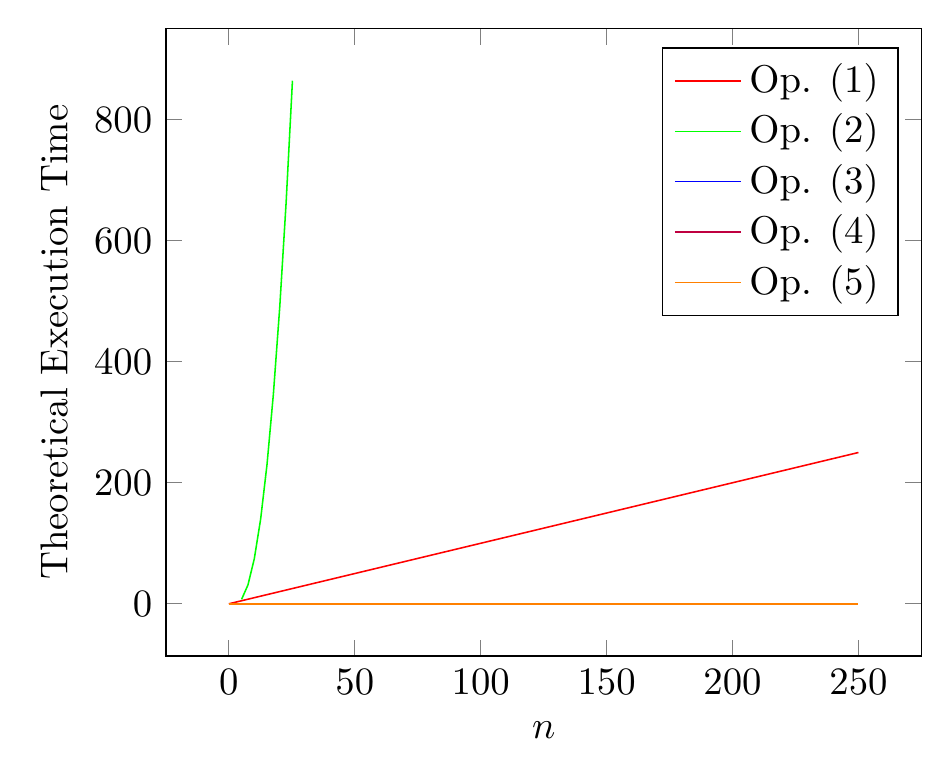
\begin{tikzpicture}[scale = 1.4]
\begin{axis}[domain=0:250, samples=100,grid=minor,
    restrict y to domain=0:1000,xlabel=$n$,ylabel=Theoretical Execution Time, 
    legend pos=north east,
    ]

\addplot [color=red]{x};
\addlegendentry{Op. (1)}

\addplot [color=green]{(1/2) * (x^2 - 1) * ((ln(x+1)/ln(2)) - 2)};
\addlegendentry{Op. (2)}

\addplot [color=blue]{0};
\addlegendentry{Op. (3)}

\addplot [color=purple]{0};
\addlegendentry{Op. (4)}

\addplot [color=orange]{0};
\addlegendentry{Op. (5)}
\end{axis}
\end{tikzpicture}
\caption{Graph of theoretical best complexities for different basic operations.}
\end{figure}


\newpage
\subsection{Worst Case}
\begin{figure}[H]
\centering
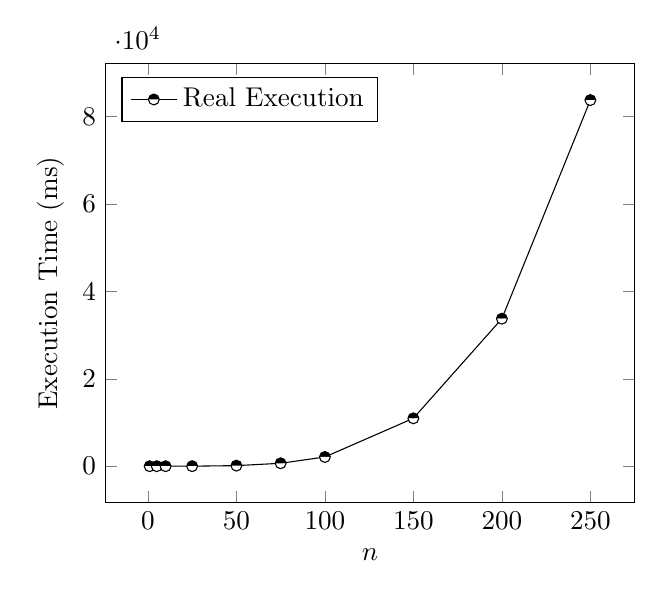
\begin{tikzpicture}[scale = 0.98]
\begin{axis}[grid=minor,
    xlabel=$n$,ylabel=Execution Time (ms), 
    legend pos=north west]
\addplot[
    color=black,
    mark=halfcircle*,
    samples=10,
    ]
    coordinates {(1,0.002861023)
 (5,0.026941299)
 (10,0.254154205)
 (25,8.384943008)
 (50,133.820772171)
 (75,671.449661255)
 (100,2112.159013748)
 (150,10967.132091522)
 (200,33765.886068344)
 (250,83805.630207062)
 };
\addlegendentry{Real Execution}
\end{axis}
\end{tikzpicture}
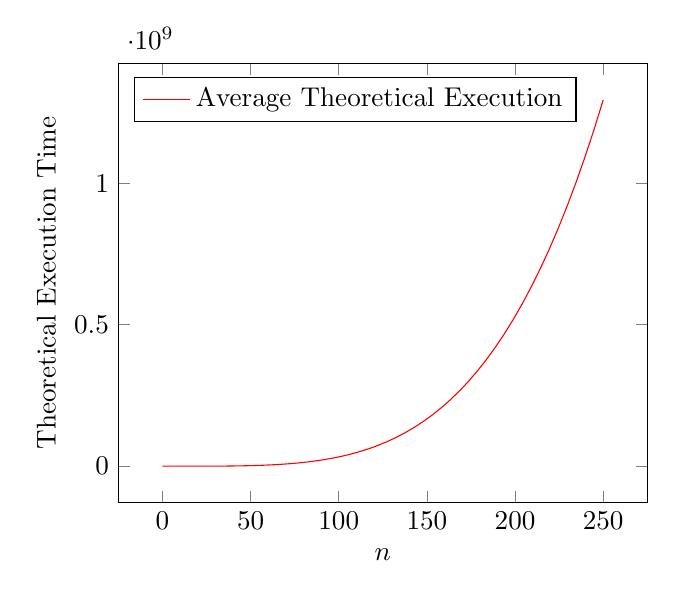
\begin{tikzpicture}[scale = 0.98]
\begin{axis}[grid=minor, xlabel=$n$,ylabel=Theoretical Execution Time,
    legend pos=north west,
    ]
\addplot [color=red, samples = 50, domain=0:250]{((x^2)/6) - ((x^3)/2) + ((x^4)/3)};
\addlegendentry{Average Theoretical Execution}
\end{axis}
\end{tikzpicture}
\caption{Side-by-side comparison of the real execution times and the correct theoretical complexity for the worst case.}
\end{figure}


\begin{figure}[H]
\centering
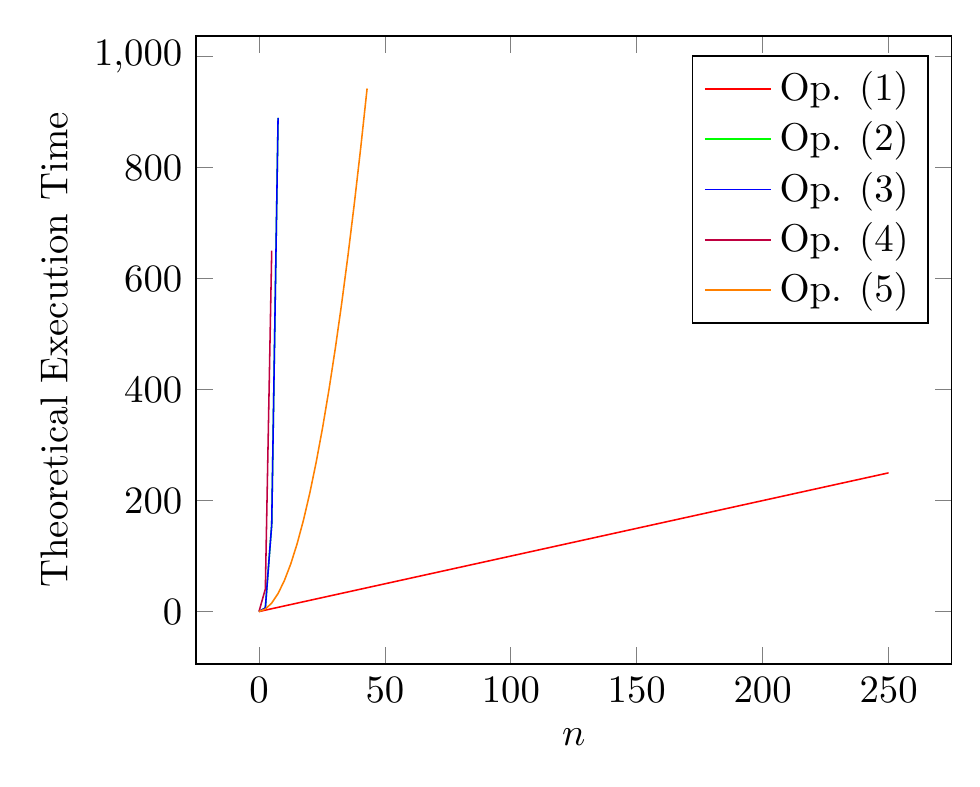
\begin{tikzpicture}[scale = 1.4]
\begin{axis}[domain=0:250, samples=100,grid=minor,
    restrict y to domain=0:1000,xlabel=$n$,ylabel=Theoretical Execution Time, 
    legend pos=north east,
    ]

\addplot [color=red]{x};
\addlegendentry{Op. (1)}

\addplot [color=green]{((x^2)/6) - ((x^3)/2) + ((x^4)/3)};
\addlegendentry{Op. (2)}

\addplot [color=blue]{((x^2)/6) - ((x^3)/2) + ((x^4)/3)};
\addlegendentry{Op. (3)}

\addplot [color=purple]{x^4};
\addlegendentry{Op. (4)}

\addplot [color=orange]{((x^2)/2) + (x/2)};
\addlegendentry{Op. (5)}
\end{axis}
\end{tikzpicture}
\caption{Graph of theoretical worst complexities for different basic operations.}
\end{figure}


\newpage
\subsection{Average Case}
\begin{figure}[H]
\centering
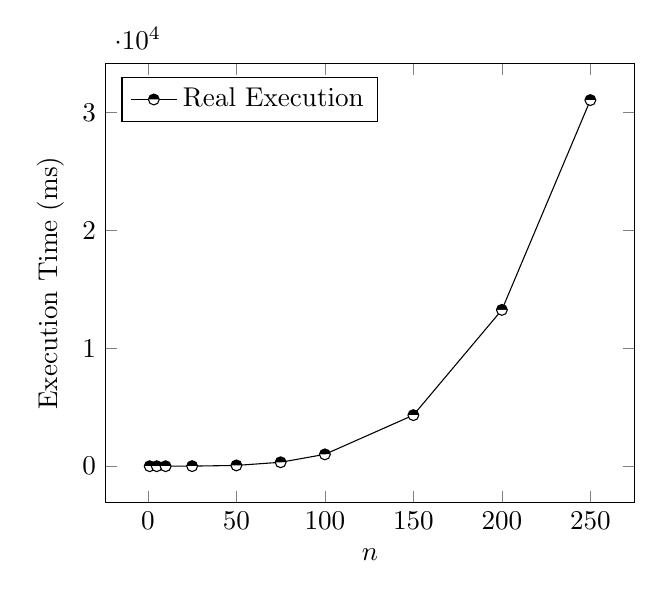
\begin{tikzpicture}[scale = 0.98]
\begin{axis}[grid=minor,
    xlabel=$n$,ylabel=Execution Time (ms), 
    legend pos=north west]
\addplot[
    color=black,
    mark=halfcircle*,
    samples=10,
    ]
    coordinates {(1,0.006437302)
 (5,0.029881795)
 (10,0.379641851)
 (25,7.709662120)
 (50,66.747744878)
 (75,334.980964661)
 (100,1006.102959315)
 (150,4331.564426422)
 (200,13257.391373316)
 (250,31049.947659175)
 };
\addlegendentry{Real Execution}
\end{axis}
\end{tikzpicture}
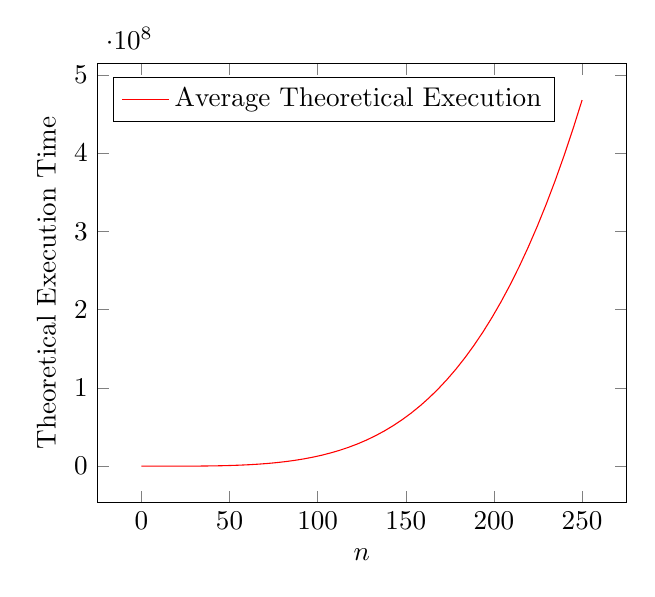
\begin{tikzpicture}[scale = 0.98]
\begin{axis}[grid=minor, xlabel=$n$,ylabel=Theoretical Execution Time,
    legend pos=north west,
    ]
\addplot [color=red, samples = 50, domain=0:250]{((x^4)/9) - ((x^3)/2) + ( ((x^3) *  (ln(x + 1)/ln(2))) /3) - ( (5*(x^2))/18) + (((x^2) * (ln(x+1)/ln(2)))/6) - ( (ln(x+1)/ln(2)) /6) + (1/3)};
\addlegendentry{Average Theoretical Execution}
\end{axis}
\end{tikzpicture}
\caption{Side-by-side comparison of the real execution times and the correct theoretical complexity for the average case.}
\end{figure}


\begin{figure}[H]
\centering
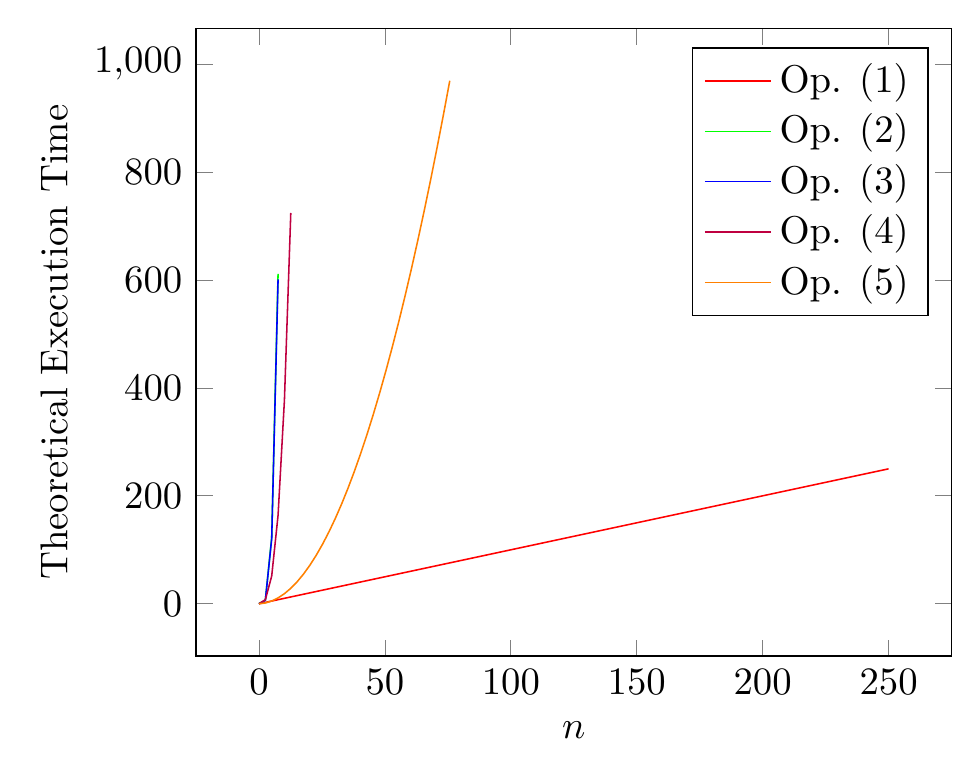
\begin{tikzpicture}[scale = 1.4]
\begin{axis}[domain=0:250, samples=100,grid=minor,
    restrict y to domain=0:1000,xlabel=$n$,ylabel=Theoretical Execution Time, 
    legend pos=north east,
    ]

\addplot [color=red]{x};
\addlegendentry{Op. (1)}

\addplot [color=green]{((x^4)/9) - ((x^3)/2) + ((((x^3) *  (ln(x + 1) / ln(2))))/3) - (((5 * (x^2)))/18) + (((x^2) * (ln(x+1)/ln(2)))/6) - (( (ln(x+1)/ln(2))/6)) + (1/3)};
\addlegendentry{Op. (2)}

\addplot [color=blue]{((x^4)/9) - ((x^3)/2) + ((x^2)/18) + (((x^3) * (ln(x+1)/ln(2)))/3)};
\addlegendentry{Op. (3)}

\addplot [color=purple]{((x^3)/3) + ((x^2)/3)};
\addlegendentry{Op. (4)}

\addplot [color=orange]{((x^2)/6) + (x/6)};
\addlegendentry{Op. (5)}
\end{axis}
\end{tikzpicture}
\caption{Graph of theoretical average complexities for different basic operations.}
\end{figure}

\newpage
\subsection{Comments on Graphs}

\indent \indent All real execution time graphs and correct theoretical complexity graphs match up. The only difference is the constant scaling between the two. The theoretical graph is about $10^4$ to $10^5$ greater in the y-axis than the real execution time graphs. Which is normal since they have different units. The scale being the same between the three cases is also a indication that our analysis was correct. \\ 
\indent The graphs of different basic operations use the complexity functions calculated in the related subsections. The actual basic operation count is used, not the complexity class. This created more variance in out graphs. \\

\textbf{Best Case} \\
\indent The best case real execution time graph rises in the same way as the correct theoretical complexity. Which indicates that our analysis was correct. The graphs for the different basic operations are not too interesting for the best case. We have one linear graph and a quadratic one, the other three graphs are just constant zero. \\

\textbf{Worst Case} \\
\indent The worst case real execution time graph rises in the same way as the correct theoretical complexity. Which indicates that our analysis was correct. Worst case graphs for different basic operations are more varied with one linear, one quadratic and three quartic graphs. This graph shows the actual complexity class difference between different polynomials. The different growth rates can be seen clearly. \\ 

\textbf{Average Case}
\indent The average case real execution time graph rises in the same way as the correct theoretical complexity. Which indicates that our analysis was correct. Average case graphs for different basic operations is the most varied of all. There is one linear, one quadratic, one cubic and two quartic graphs. The average case graphs, especially the quartic ones, have more terms in them and result in a set of graphs which are more varied than the other cases. \\ 


\end{document}
